% Setting all the margins and boxes
\newgeometry{
letterpaper,
top=2cm,
bottom=2cm,
footskip=1.5cm,
inner=2cm,
outer=2cm,
marginparwidth=0cm
}

\changefontsize{12pt}

% Positioning page-numbers
\pagestyle{fancy}
\fancyhf{}
\fancyfoot[L]{
    \selectlanguage{english}
    \fontfamily{qag}{\selectfont{
        \Huge 20
    }}
    \selectlanguage{russian}
}
\renewcommand{\headrulewidth}{0pt} % Because of fancyhdr, a line appears at the top of the page

\begin{multicols}{2}

\begin{figure}[H]
    \centering
    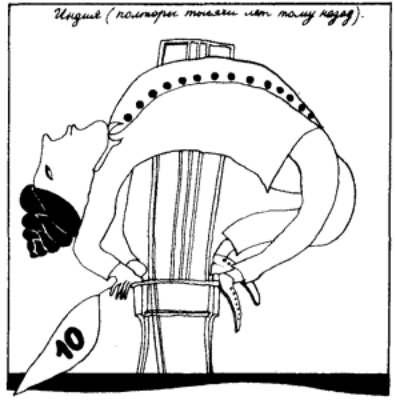
\includegraphics[width=0.9\linewidth]{kvant_89-lying.png}
    \label{fig:kvant_89-lying}
\end{figure}

\noindent ния. Миллион они называли \guillements{коти}, сто миллионов - \guillements{врнда}, а в легендах о Будде рассказывалось, как он давал имена еще б\`{о}льшим числам - плоть до числа, записываемого единицей с пятьюдесятью нулями.

Но в Европе после падения античной науки не знали  названий разрядов чисел, следующих за тысячей. Число 999 999 европейские математики еще могли прочесть, а дальше они считать не умели. В 1271-1275 годах венецианский купец Марко Поло совершил неслыханное для той поры путешествие. Пройдя северным побережьем Черного моря, он пересек Волгу, бескрайние азиатские степи и Великим шелковым путем добрался до Китая. Здесь он прожил много лет, наблюдая то, о чем тогдашние европейцы и понятия не имели: полеты пороховых ракет, книгопечатание, изготовление фарфора.

Когда он снова оказался в Венеции, рассказам не было конца. И чаще всего в рассказах Марко Поло повторялось слово \guillements{миллионе} - большая тысяча. Так он назвал тысячу тысяч. Недоверчивые венецианцы прозвали путешественника Марко Миллионе и думали, что он их обманывает. Только через несколько столетий, когда европейцы лучше познакомились с Китаем, они узнали, что рассказы Поло были правдивыми.

В XV веке французский математик Никола Шюке по созвучию с миллионом ввел слово \guillements{биллион}, которое означает миллион миллионов. Что бы записать биллион, надо после единицы поставить 12 нулей. Приставка \guillements{би} по-латыни означала \guillements{второй} (в театрах кричат \guillements{бис}, когда хотят повторения). Поэтому \guillements{биллион} можно прочесть и так: \guillements{второй миллион}. Миллион биллионов назвали \guillements{триллионом}, а миллион триллионов получил название \guillements{квадриллион} (от латинского слова \guillements{кварта} - \guillements{четыре}).

В США, Англии и Германии принята иная система названий чисел. По этой системе тысячу миллионов называют миллиардом или биллионом, тысячу биллионов - триллионом, тысячу триллионов - квадриллионом. Эту систему названий используют и в нашей стране. Вот названия некоторых громадных чисел с указанием числа нулей после единицы в двух системах:


\begin{table}[H]
    \centering
    \begin{tabular}{|l|c|c|}
         \hline
         \; & Франция & \thead{СССР, США, \\ Германия, Англия} \\
         \hline
         Миллион     & 6  & 6  \\
         Биллион     & 12 & 9  \\
         Триллион    & 18 & 12 \\
         Квадриллион & 24 & 15 \\
         Квинтиллион & 30 & 18 \\
         Секстиллион & 36 & 21 \\
         Септиллион  & 42 & 24 \\
         Окталлион   & 48 & 27 \\
         Нонакаллион & 54 & 30 \\
         Декаллион   & 60 & 33 \\
         \hline
    \end{tabular}
    \label{tab:millions_table}
\end{table}

В школе этих названий уже не изучают, да они и не слишком нужны. В газетах мы часто читаем, что та или иная фабрика выпустила столько-то миллионов метров ткани или такая-то гидростанция дала столько-то миллиардов киловатт-часов электроэнергии. Триллионы встречаются в газетах, когда пишут о бюджетах крупнейших государств. А вот название \guillements{квадриллион} в газетах не попадается - вряд ли есть что-нибудь на земном шаре, что исчислялось бы квадриллионами.

Только в науке оказываются нужны такие числа. В 16 граммах воздуха содержится примерно септил-

\end{multicols}
